\documentclass[10pt,letterpaper]{article}
\usepackage{ccn}
\usepackage[T1]{fontenc}
\usepackage{amsmath,amssymb,graphicx,booktabs,tabularx,array,enumitem,float}
\usepackage[round,authoryear]{natbib}
\usepackage[hidelinks]{hyperref}
\usepackage{microtype}

% Every number below is a macro generated from the result files (see review/make_review_numbers.py).
% generated by experiments/make_numbers.py - do not edit
\newcommand{\ablNoActConst}{0.38}
\newcommand{\ablNoActGrid}{38\%}
\newcommand{\ablNoActHex}{2}
\newcommand{\ablNoActMin}{-0.19}
\newcommand{\ablNoActModules}{6}
\newcommand{\ablNoActNeff}{12.5}
\newcommand{\ablNoActNeg}{0.005}
\newcommand{\ablNoFunConst}{0.34}
\newcommand{\ablNoFunGrid}{0\%}
\newcommand{\ablNoFunHex}{0}
\newcommand{\ablNoFunMin}{0.99}
\newcommand{\ablNoFunModules}{1}
\newcommand{\ablNoFunNeff}{1.0}
\newcommand{\ablNoFunNeg}{0.000}
\newcommand{\ablNoPosConst}{0.02}
\newcommand{\ablNoPosGrid}{2\%}
\newcommand{\ablNoPosHex}{0}
\newcommand{\ablNoPosMin}{-3.16}
\newcommand{\ablNoPosModules}{20}
\newcommand{\ablNoPosNeff}{7.4}
\newcommand{\ablNoPosNeg}{0.498}
\newcommand{\actErrMax}{$5\times10^{-13}$}
\newcommand{\actRankMin}{1\times10^{-5}}
\newcommand{\angleBandFrac}{32\%}
\newcommand{\angleBandOfInterior}{38\%}
\newcommand{\angleInterior}{83\%}
\newcommand{\angleMeasBand}{0\%}
\newcommand{\angleMeasLow}{50\%}
\newcommand{\angleMeasMedian}{5.8}
\newcommand{\angleMeasPairs}{6}
\newcommand{\angleMeasRuns}{4}
\newcommand{\angleRef}{4.0}
\newcommand{\angleRefMu}{0.030}
\newcommand{\angleRefNu}{0.14}
\newcommand{\angleScanMax}{30}
\newcommand{\angleScanMin}{1.0}
\newcommand{\angleThreeA}{3.5}
\newcommand{\angleThreeB}{3.5}
\newcommand{\baseConst}{1.06}
\newcommand{\baseGrid}{9\%}
\newcommand{\baseHex}{0.3}
\newcommand{\baseModules}{4.7}
\newcommand{\baseModulesSd}{1.5}
\newcommand{\baseNeff}{7.0}
\newcommand{\baseNeg}{0.005}
\newcommand{\baseSeeds}{9}
\newcommand{\lamNFinal}{$10^{-8}$}
\newcommand{\lbFinalMean}{3.06}
\newcommand{\lpFinalMean}{0.0001}
\newcommand{\mainHighGridA}{100\%}
\newcommand{\mainHighGridB}{100\%}
\newcommand{\mainHighGridFrac}{100\%}
\newcommand{\mainHighGridFracWin}{87\%}
\newcommand{\mainHighHexA}{1}
\newcommand{\mainHighHexB}{1}
\newcommand{\mainHighHexMean}{1.0}
\newcommand{\mainHighInModules}{100\%}
\newcommand{\mainHighModulesA}{1}
\newcommand{\mainHighModulesB}{1}
\newcommand{\mainHighModulesMax}{1}
\newcommand{\mainHighModulesMean}{1.0}
\newcommand{\mainHighModulesMin}{1}
\newcommand{\mainHighNRuns}{2}
\newcommand{\mainHighNegMass}{0.010}
\newcommand{\mainHighSizesA}{64}
\newcommand{\mainHighSizesB}{64}
\newcommand{\mainLowGridA}{14\%}
\newcommand{\mainLowGridB}{0\%}
\newcommand{\mainLowGridC}{0\%}
\newcommand{\mainLowGridFrac}{5\%}
\newcommand{\mainLowGridFracWin}{11\%}
\newcommand{\mainLowHexA}{0}
\newcommand{\mainLowHexB}{0}
\newcommand{\mainLowHexC}{0}
\newcommand{\mainLowHexMean}{0.0}
\newcommand{\mainLowInModules}{99\%}
\newcommand{\mainLowModulesA}{3}
\newcommand{\mainLowModulesB}{3}
\newcommand{\mainLowModulesC}{6}
\newcommand{\mainLowModulesMax}{6}
\newcommand{\mainLowModulesMean}{4.0}
\newcommand{\mainLowModulesMin}{3}
\newcommand{\mainLowNRuns}{3}
\newcommand{\mainLowNegMass}{0.008}
\newcommand{\mainLowSizesA}{38/24/2}
\newcommand{\mainLowSizesB}{35/19/10}
\newcommand{\mainLowSizesC}{18/16/11/8/6/4}
\newcommand{\nJobs}{60}
\newcommand{\nRunsFinished}{60}
\newcommand{\nTests}{20}
\newcommand{\oneDDev}{0.26}
\newcommand{\oneDFund}{0.53}
\newcommand{\oneDMeanRms}{0.66}
\newcommand{\oneDNeff}{6.1}
\newcommand{\oneDNeg}{6.8\%}
\newcommand{\oneDNull}{0.11}
\newcommand{\oneDShare}{29\%}
\newcommand{\oneDUniDev}{0.29}
\newcommand{\oneDUniMeanRms}{0.55}
\newcommand{\oneDUniShare}{8\%}
\newcommand{\sharpCIHi}{3.66}
\newcommand{\sharpCILo}{-0.69}
\newcommand{\sharpNMod}{30}
\newcommand{\sharpNRuns}{25}
\newcommand{\sharpR}{0.35}
\newcommand{\sharpSlope}{1.47}
\newcommand{\sharpSpearman}{0.59}
\newcommand{\sigmaLarge}{1.0}
\newcommand{\sigmaLargeModules}{1.0}
\newcommand{\sigmaSmall}{0.1}
\newcommand{\sigmaSmallModules}{9.5}
\newcommand{\sigmaTwoLarge}{1.0}
\newcommand{\sigmaTwoLargeHex}{1.0}
\newcommand{\sigmaTwoLargeModules}{1.0}
\newcommand{\sigmaTwoSmallModules}{11.5}
\newcommand{\trainMinLong}{15}
   % written by numpy_impl/experiments/make_numbers.py
% generated by make_review_numbers.py - do not edit
\newcommand{\auditCommit}{7db3147}
\newcommand{\auditGrad}{$5.1\times10^{-11}$}
\newcommand{\auditLoss}{$2.8\times10^{-13}$}
\newcommand{\auditPassed}{passes}
\newcommand{\jCtlFifty}{0.0961}
\newcommand{\jCtlFiftyFrac}{4\%}
\newcommand{\jCtlOneFifty}{0.0274}
\newcommand{\jCtlOneFiftyFrac}{34\%}
\newcommand{\jCtlRel}{$7\times10^{-8}$}
\newcommand{\jCtlSixHundred}{0.00644}
\newcommand{\jCtlSixHundredFrac}{100\%}
\newcommand{\jCtlTarget}{0.02}
\newcommand{\jDiagBaseNormHi}{0.0301}
\newcommand{\jDiagBaseNormLo}{0.0209}
\newcommand{\jDiagBaseScoreHi}{0.065}
\newcommand{\jDiagBaseScoreLo}{0.048}
\newcommand{\jDiagBaseSeeds}{3}
\newcommand{\jDiagBothMet}{0}
\newcommand{\jDiagMinutes}{71}
\newcommand{\jDiagRuns}{9}
\newcommand{\jDiagSteps}{150\,000}
\newcommand{\jDiagTabNormHi}{3.87}
\newcommand{\jDiagTabNormLo}{1.77}
\newcommand{\jDiagTabScoreHi}{-0.037}
\newcommand{\jDiagTabScoreLo}{-0.123}
\newcommand{\jDiagTabSeeds}{3}
\newcommand{\jDiagVarNormHi}{0.0243}
\newcommand{\jDiagVarNormLo}{0.0148}
\newcommand{\jDiagVarScoreHi}{0.101}
\newcommand{\jDiagVarScoreLo}{0.067}
\newcommand{\jDiagVarSeeds}{3}
\newcommand{\jRefHalfNeg}{3.6\%}
\newcommand{\jRefHalfNorm}{0.030}
\newcommand{\jRefHalfNormMet}{missed}
\newcommand{\jRefHalfScore}{0.050}
\newcommand{\jRefMinutes}{9}
\newcommand{\jRefTenthNeg}{5.1\%}
\newcommand{\jRefTenthNorm}{0.019}
\newcommand{\jRefTenthNormMet}{met}
\newcommand{\jRefTenthScore}{0.009}
\newcommand{\xBaseLamAtFloor}{8}
\newcommand{\xBaseLamRuns}{8}
\newcommand{\xBaseLbHi}{1.9}
\newcommand{\xBaseLbLo}{0.8}
\newcommand{\xCpuHours}{5.3}
\newcommand{\xHalfHexA}{1}
\newcommand{\xHalfHexB}{0}
\newcommand{\xHalfModulesA}{1}
\newcommand{\xHalfModulesB}{2}
\newcommand{\xLamMainAll}{all}
\newcommand{\xLbMainMax}{5.7}
\newcommand{\xLbMainMin}{1.1}
\newcommand{\xLooseOneGrid}{100\%}
\newcommand{\xLooseOneHex}{1}
\newcommand{\xLooseOneModules}{1}
\newcommand{\xLtenHexH}{0}
\newcommand{\xLtenHexN}{0}
\newcommand{\xLtenModulesH}{3}
\newcommand{\xLtenModulesN}{3}
\newcommand{\xMainLowGridMax}{14\%}
\newcommand{\xMainLowTotalHex}{0}
\newcommand{\xMainLowTotalModules}{12}
\newcommand{\xRunsTimed}{60}
\newcommand{\xSpacingLoose}{4.2}
\newcommand{\xSpacingTight}{3.7}
\newcommand{\xTightLowGrid}{22\%}
\newcommand{\xTightLowHex}{0}
\newcommand{\xTightLowLam}{0.36}
\newcommand{\xTightLowLb}{0.026}
\newcommand{\xTightLowModules}{6}
\newcommand{\xTightOneGrid}{0\%}
\newcommand{\xTightOneHex}{0}
\newcommand{\xTightOneLam}{2.0}
\newcommand{\xTightOneLb}{0.021}
\newcommand{\xTightOneModules}{1}
   % written by review/make_review_numbers.py (NumPy extras, JAX results, cross-check)

\title{Actionability as an Explanation of Grid Cells:\\A Critical Review and Reproduction of Dorrell et al. (2023)}
\author{{\large\bf Tafara Chibanda (2683459)}\\University of the Witwatersrand
\And {\large\bf Nathan Le Roux (2717495)}\\University of the Witwatersrand}

\begin{document}
\maketitle

\section{Summary}
Dorrell et al.\ (2023, ICLR) ask why the brain would represent two-dimensional position with grid cells. Their answer is that a spatial code should be \emph{actionable}: every movement (a step north, then east, and so on) should change the population activity by the same matrix wherever the animal starts, so that a route never travelled can still be predicted. Representation theory then forces each neuron's tuning to be a sum of sinusoids of position, leaving only the sinusoids' amplitudes and wave vectors to be learned. The authors choose them by gradient descent (64 neurons) so that the codes of distant places stay distinct, while firing is kept non-negative and bounded. The optimum, they report, is several modules of roughly hexagonal grid cells. They explain this with analytic and heuristic arguments: non-negativity needs a constant offset or harmonically related frequencies, which gives a lattice of frequencies; the animal's occupancy and the resolution it needs select a ring of useful frequencies that a hexagonal lattice fills most densely; and a small neural length scale $\sigma$ favours non-harmonic frequencies, hence several modules. Three predictions follow (module size against field width, small offsets between module orientations, and changes with room shape), compared informally with \citet{stensola2012}. We read the optimality claim as a numerically supported heuristic rather than a proof, since the paper's Appendix~G calls the problem non-convex; this is the point in our understanding we are least sure of.

\section{Originality}
Earlier accounts work at other levels. Continuous-attractor models \citep{burak2009} hand-tune a circuit that integrates velocity; efficient-coding analyses, as the authors note, assume grid-like tuning. \citet{sorscher2019} obtain hexagonal grids from non-negativity and a place-cell read-out target and, in the authors' view (Appendix~H.2), modules only through a quantisation effect. Closest is \citet{gao2021}: they also use a position-independent linear update (a group representation), but add an isotropy term that favours hexagons directly and obtain several modules only by imposing block-diagonal updates. Dorrell et al.\ keep the linear action, drop the isotropy term, derive hexagons from the band of useful spatial frequencies, and derive modules from~$\sigma$. The distinctive contributions are therefore (i) a reduction, through representation theory, to a small interpretable family of codes, (ii) modules without hand-built structure, and (iii) quantitative predictions.

The weaknesses follow from the framework. Requiring a location-independent \emph{linear} action is a substantive restriction, so periodic tuning is largely a consequence of the formulation, and ``grid cells from minimal constraints'' means hexagonal and modular codes \emph{within} linear-action models. The claim that isotropy is unnecessary (Appendix~H.1) is argued but never tested by running the authors' objective with and without it, and there is no head-to-head comparison with \citet{sorscher2019}.

\emph{Level of abstraction.} The paper is computational: it has no spiking, learning rule, velocity input or noise. That is more abstract than attractor or trained-network models, and more general in what it can represent (any variable whose transformations form a group, as on the circle, sphere and 3-D space of Appendix~M), but less general in its update rule. We agree with this choice for a ``why'' question, because it lets the authors derive rather than fit. The cost is that the link to attractor circuits, which they leave as future work, stays open.

\section{Clarity}
The paper is well organised. Section~2 builds the idea on a circle before the plane, Figure~4A shows the frequency-ring argument at a glance, Figure~6 shows every neuron of the main population, and the authors are candid about simplifications (``this is a bad loss'', Section~3.1). Our difficulties were specific:
\begin{enumerate}[leftmargin=1.4em,itemsep=0pt,topsep=2pt,parsep=0pt]
\item Table~B.3 gives the settings of Figure~2B only. Figures~8 and~9 change $\sigma$, $l$ and the number of steps and rescale the initial constraint weights with the loss size, without giving values.
\item The number of frequencies $D$ and the initial variances (``as in Table~B.3'') are not in the table.
\item The norm target $k_n=4$ is a log-target (equation~26), but the equation~25 penalty is an average squared error that is small when the constraint holds. A target of $e^{4}\approx55$ is far above the values of any sensible code and, in our runs, switched the constraint off (see Reproducibility).
\item Equation~22 normalises by a \emph{sum} over $M$ sampled points while the main text uses expectations, so the numerical meaning of $\sigma$ depends on $M$.
\item Figure~9 counts ``modules'' and Figure~8 judges ``hexagonal'' without saying how, and the Figure~2B caption omits $\sigma$, $N$ and $l$.
\item Figure~5 holds nine panels, and its comparisons with data (5B, 5E, 5I) are by eye, without an effect size.
\end{enumerate}
Tafara's reading of the public code (commit 940659e, \href{https://github.com/WilburDoz/ICLR_Actionable_Reps}{authors' repository}) found that its norm routine aggregates unnormalised responses where equation~25 uses normalised ones, and that its \texttt{sigma\_sq} argument must be distinguished from the paper's $\sigma$. These point to a need for per-figure configuration files, not to errors in the reported results.

\section{Quality}
\emph{Strengths.} Each ingredient is tied to a mechanism that makes a checkable statement: non-negativity forces harmonics and a constant offset, the two spatial scales select a ring of frequencies, and $\sigma$ sets how many modules arise. The last held in our runs: at $l=0.5$ the number of modules rose from \sigmaLargeModules{} at $\sigma=\sigmaLarge$ to \sigmaSmallModules{} at $\sigma=\sigmaSmall$ (Table~\ref{tab:verdict}). The authors also volunteer limits (Appendix~B.4.2: ``the more modules the less hexagonal''; their data comparisons are ``rudimentary'').

\emph{Weaknesses.} (1) Optimality is heuristic: Appendix~G calls the problem non-convex, and the evidence is gradient descent from random starts, which varies with the seed. At $\sigma=0.2$, nine 50k-step runs gave \baseModules{}$\pm$\baseModulesSd{} modules with \baseHex{} hexagonal per run on average; three runs at the paper's 150k steps gave \mainLowModulesA, \mainLowModulesB{} and \mainLowModulesC{} modules, none hexagonal. Figure~2B is thus a favourable instance, and ``several hexagonal modules'' is the weakest part of the central result. (2) ``Minimal'' rests on ablations on a small torus (Appendix~I). On the plane, removing non-negativity or the functional term destroyed grid structure in our runs, but removing actionability did not (\ablNoActGrid{} of cells still scored above 0.3), so a grid score alone cannot separate lattices from bumpy patterns. (3) The hexagonal outcome appears to depend on how the bounded-activity constraint is enforced (Reproducibility). Appendix~B.4 says dependence on optimiser settings ``does not seem deeply worrying''; this one changes the result. (4) The predictions are weakly constrained. The scaling $N\propto(\nu/\mu)^2$ is supported in sign but not decisively (slope \sharpSlope, 95\% bootstrap interval $\sharpCILo$ to $\sharpCIHi$, \sharpNMod{} modules), and the $\sim4^\circ$ offset depends on $\mu$ and $\nu$ values that are not reported: only \angleBandFrac{} of the values we scanned give 3--8$^\circ$.

\emph{Abstraction.} We agree with the level for the question ``what makes a code useful'', less so for the biological reading. The optimiser sees explicit position samples and a global loss, non-negativity and boundedness are penalties, and nothing says how a circuit would store a separate $N\times N$ matrix $T(\Delta x)$ for every displacement. An optimal code is not shown to be learnable, or robust to noise.

\section{Significance}
\emph{Influence.} The paper gives a template: choose a variable, write down the group of its transformations, add biological and functional constraints, and read off the code. The authors already apply it to circles, spheres and 3-D space; for 3-D they suggest that irregular fields in rats and bats mean that animals give up actionability there, an intriguing claim resting on a thin argument (Appendix~M). For machine learning, the principle that a representation should let a system predict the consequences of its actions is broadly useful. The theory complements circuit models: it says which codes are useful, and mechanistic models ask whether plausible networks can implement them. Recordings showing toroidal population structure in grid modules \citep{gardner2022} make that relationship timely.

\emph{Theory--experiment loop.} The theory was motivated by known grid properties (hexagons, modules) and returns predictions, but these need sharper tests than visual comparison with \citet{stensola2012}. Three experiments follow directly. (1)~\emph{Room geometry.} Record the same module in a square and then a rectangle, fit any free parameters in the first room only, and predict which cells keep their scale and which shift. Separate physical walls from sampled occupancy, because the theory enters through $p(x)$. (2)~\emph{Module offsets.} Measure $\mu$ and $\nu$ for each module pair, compute the predicted offset (in our re-implementation it depends strongly on both), and compare with a null of random orientations, whose mean offset is $15^\circ$. (3)~\emph{Actionability itself.} The core assumption, one position-independent linear map per displacement, has not been tested directly. With simultaneously recorded neurons of one module, fit a map per displacement on part of the arena and predict held-out population vectors; position-dependent or nonlinear updates, as in attractor models, would fail where actionability succeeds. Failures would feed back into the model, by adding sensory input or noise, as the authors suggest, or the isotropy term of \citet{gao2021}, which the authors say (Appendix~H.1) may be needed to make many modules hexagonal. Our runs, where multi-module codes were rarely hexagonal, support trying it. Because several models produce grids, experiments should target where their predictions differ, not whether grids appear.

\section{Reproducibility}
We built two implementations. Nathan's (NumPy, hand-derived gradients checked against finite differences, \nJobs{} training runs) was written from the paper's text only; the authors' code was deliberately not read. Tafara's (JAX, automatic differentiation, two reference runs and nine controlled \jDiagSteps-step runs) inspected the authors' public code (commit 940659e) when choosing initialisation and optimiser conventions, so the two used different information. On identical float64 inputs their loss terms agree to \auditLoss{} and, after aligning the functional weight, their directional derivatives to \auditGrad{}: both optimise the same equations. Table~\ref{tab:verdict} lists every claim we tested.

\emph{What held.} A single hexagonal module at large $\sigma$ (both 150k-step runs at $\sigma=\sigmaLarge$, and $\sigma=0.7$), and a module count that grows as $\sigma$ falls (Figure~\ref{fig:sigma}).

\emph{What did not.} (i)~Figure~2B: at $\sigma=0.2$ and 150k steps we found \xMainLowTotalModules{} modules in three runs, none hexagonal (at most \xMainLowGridMax{} of cells with grid score above 0.3; Figure~\ref{fig:main}). (ii)~The single hexagonal module of Figure~8 ($\sigma=0.4$, $l=0.5$): Tafara's 150k-step runs gave elongated periodic cells (median grid score \jRefHalfScore; Figure~\ref{fig:jaxcomp}), and Nathan's 50k-step runs gave one hexagonal module in one of two seeds. With $l=0.1$, $N=100$ gave \xLtenModulesH{} modules, none hexagonal. (iii)~The $\sim4^\circ$ module offset: \angleMeasPairs{} pairs of our hexagonal modules (\angleMeasRuns{} runs) gave none in 3--8$^\circ$. (iv)~The 1-D lattice of Section~3.1 was only partly seen: non-negativity was reached with a smaller offset than one sinusoid needs (mean/RMS \oneDMeanRms{} against 0.82), but only \oneDShare{} of the power lay within 0.1 of an integer multiple of the fundamental (20\% for random ratios).

\emph{The norm constraint.} Table~B.3 is not sufficient to reproduce Figure~2B: it omits $D$ and the initial variances, and its norm target, taken literally ($k_n=4$), leaves the constraint inactive. In all five main NumPy runs the norm multiplier decayed to its floor and the training norm loss ended at \xLbMainMin--\xLbMainMax{}; Tafara's literal-target runs ended at held-out errors of \jDiagTabNormLo--\jDiagTabNormHi. A tight target ($\approx0.02$) does enforce the constraint, and in both implementations it gave elongated, banded cells instead of hexagons (Figure~\ref{fig:montage}): Nathan's $\sigma=1$ run gave \xTightOneHex{} hexagonal modules where the literal target gave \xLooseOneHex{} (one seed, 50k steps), and all three of Tafara's seeds gave median grid scores of only \jDiagBaseScoreLo--\jDiagBaseScoreHi{} (Figure~\ref{fig:diag}). Tafara's control adds that a hand-built hexagonal code incurs a mean norm penalty of \jCtlOneFifty{} with 150 sampled points, above the 0.02 target (Figure~\ref{fig:control}). The hexagonal result therefore seems to depend on how loosely boundedness is enforced. This is a hypothesis from few runs, not a conclusion.

\emph{Limits.} We ran two to nine seeds per setting, our thresholds for ``module'' and ``hexagonal'' are not the paper's, and grid scores are descriptive. We did not attempt room geometry, 3-D, or the paper's torus ablations. These results do not show that the paper is wrong, only that its text alone does not fix the outcome.

\begin{thebibliography}{5}
\bibitem[Burak and Fiete(2009)]{burak2009}
Burak, Y., \& Fiete, I. R. (2009).
Accurate path integration in continuous attractor network models of grid cells.
\emph{PLoS Computational Biology, 5}(2), e1000291.
\url{https://doi.org/10.1371/journal.pcbi.1000291}
\bibitem[Gao et al.(2021)]{gao2021}
Gao, R., Xie, J., Wei, X.-X., Zhu, S.-C., \& Wu, Y. N. (2021).
On path integration of grid cells: Group representation and isotropic scaling.
\emph{Advances in Neural Information Processing Systems, 34}.
\url{https://arxiv.org/abs/2006.10259}
\bibitem[Gardner et al.(2022)]{gardner2022}
Gardner, R. J., Hermansen, E., Pachitariu, M., Burak, Y., Baas, N. A., Dunn, B. A., Moser, M.-B., \& Moser, E. I. (2022).
Toroidal topology of population activity in grid cells.
\emph{Nature, 602}, 123--128.
\url{https://doi.org/10.1038/s41586-021-04268-7}
\bibitem[Sorscher et al.(2019)]{sorscher2019}
Sorscher, B., Mel, G. C., Ganguli, S., \& Ocko, S. A. (2019).
A unified theory for the origin of grid cells through the lens of pattern formation.
\emph{Advances in Neural Information Processing Systems, 32}.
\bibitem[Stensola et al.(2012)]{stensola2012}
Stensola, H., Stensola, T., Solstad, T., Fr{\o}land, K., Moser, M.-B., \& Moser, E. I. (2012).
The entorhinal grid map is discretized.
\emph{Nature, 492}(7427), 72--78.
\end{thebibliography}

\section{Author contributions and AI use}
Nathan Le Roux ran the NumPy implementation and its \nJobs-run campaign. Tafara Chibanda ran the JAX implementation, the controlled diagnostics, the constructed control and the equation audit, and prepared the first review draft. Claude (Anthropic) wrote the NumPy code, tests and analysis scripts and drafted this merged review from both authors' material and the result files; OpenAI Codex assisted with the JAX code, tests, analysis and the earlier review draft. This statement accompanies the Wits Science Faculty AI declaration. The authors take responsibility for everything submitted.

\clearpage
\onecolumn
\renewcommand{\thetable}{A\arabic{table}}\renewcommand{\thefigure}{A\arabic{figure}}
\setcounter{table}{0}\setcounter{figure}{0}
\section*{Appendix: tables}
\renewcommand{\arraystretch}{1.05}
\begin{table}[H]
\centering\footnotesize
\caption{Every claim of the paper that we tested, with what we found (NumPy: Nathan's implementation, \nJobs{} runs, 64 neurons, $L=1$, steps as stated; JAX: Tafara's implementation, 150\,000 steps). Section and figure numbers refer to the paper. ``Hexagonal'' is judged from the autocorrelogram of the whole plane (six nearest peaks within $15^\circ$ of a hexagon, lengths within 25\%, gridness above 0.3), thresholds that are ours; JAX grid scores are descriptive.}
\label{tab:verdict}
\begin{tabularx}{\linewidth}{@{}>{\raggedright\arraybackslash}p{4.3cm}>{\raggedright\arraybackslash}X>{\raggedright\arraybackslash}p{2.7cm}@{}}
\toprule
Claim (paper) & What we found & Verdict\\
\midrule
One hexagonal module at large $\sigma$ (Figs.~4B, 8, 9) & NumPy, 150k steps, two runs at $\sigma=\sigmaLarge$: modules \mainHighModulesA{} and \mainHighModulesB{}, hexagonal modules \mainHighHexA{} and \mainHighHexB{}; also $\sigma=0.7$ (and $l=0.2$) & Held\\
More modules as $\sigma$ falls (Sec.~3.3, Fig.~9) & NumPy, $l=0.5$, 50k steps: \sigmaLargeModules{} modules at $\sigma=\sigmaLarge$ rising to \sigmaSmallModules{} at $\sigma=\sigmaSmall$ & Held\\
Several hexagonal modules at $\sigma=0.2$ (Fig.~2B) & NumPy, 150k steps, 3 seeds: \mainLowModulesA/\mainLowModulesB/\mainLowModulesC{} modules, \xMainLowTotalHex{} hexagonal, at most \xMainLowGridMax{} of cells above 0.3. 50k steps, \baseSeeds{} seeds: \baseModules{} modules, \baseHex{} hexagonal per run & Not reproduced\\
One hexagonal module at $\sigma=0.4$, $l=0.5$, $N=64$ (Fig.~8) & JAX, 150k steps: median grid score \jRefHalfScore{} (seed 0), \jDiagBaseScoreLo--\jDiagBaseScoreHi{} over \jDiagBaseSeeds{} seeds, elongated periodic cells. NumPy, 50k steps: hexagonal in one of two seeds (\xHalfModulesA{} and \xHalfModulesB{} modules) & Not reproduced (mixed)\\
$N=100$ gives a hexagonal module at $l=0.1$ (Fig.~8) & NumPy, 50k steps, one run: \xLtenModulesH{} modules, \xLtenHexH{} hexagonal ($N=64$: \xLtenModulesN{} modules, \xLtenHexN{} hexagonal) & Not reproduced (one run)\\
Non-negativity gives a harmonic lattice (Sec.~3.1, Fig.~3C) & NumPy, 1-D line, simplified loss: mean/RMS \oneDMeanRms{} (single sinusoid: 0.82), \oneDNeg{} of values negative; \oneDShare{} of power within 0.1 of an integer multiple (random: 20\%) & Partly\\
All three ingredients needed (App.~I, Fig.~15) & NumPy, 50k steps, one run each: without non-negativity \ablNoPosModules{} modules, none hexagonal, \ablNoPosGrid{} of cells above 0.3; without the functional term \ablNoFunModules{} module, \ablNoFunGrid{}; without actionability ($D=96$) \ablNoActModules{} modules, \ablNoActHex{} hexagonal, \ablNoActGrid{} of cells above 0.3 & 2 of 3\\
$N\propto(\nu/\mu)^2$ (Sec.~4.1) & NumPy: log--log slope \sharpSlope{} (95\% bootstrap interval $\sharpCILo$ to $\sharpCIHi$; paper: 2), Spearman \sharpSpearman, \sharpNMod{} hexagonal modules from \sharpNRuns{} runs & Consistent, not decisive\\
Neighbouring modules differ by $\sim4^\circ$ (Sec.~4.2, App.~K) & NumPy re-implementation of App.~K gives \angleRef$^\circ$ only for $(\mu,\nu)=(\angleRefMu,\angleRefNu)$, values the paper does not give; \angleBandFrac{} of scanned values fall in 3--8$^\circ$. Measured: \angleMeasPairs{} pairs, none in 3--8$^\circ$, median \angleMeasMedian$^\circ$ (null 15$^\circ$) & Not reproduced\\
Table~B.3 suffices for Fig.~2B & $D$ and initial variances missing. Literal $k_n=4$: multiplier at its floor in \xBaseLamAtFloor{} of \xBaseLamRuns{} 50k-step runs and in all five main runs; norm loss \xLbMainMin--\xLbMainMax{} (main) & Not sufficient\\
Same equations in both implementations & Loss terms agree to \auditLoss, directional derivatives to \auditGrad{} (float64, shared fixture, NumPy core at commit \auditCommit; audit \auditPassed) & Agree\\
Not attempted & Room-geometry predictions (Sec.~4.3, Fig.~5F--I), the 3-D case (Fig.~19), the torus ablations as drawn in Fig.~15 & ---\\
\bottomrule
\end{tabularx}
\end{table}

\begin{table}[H]
\centering\footnotesize
\caption{The norm target in both implementations. Targets are on the loss of equation~25: the literal target is $e^{k_n}$ with $k_n=4$, the tight ones are $e^{-4}\approx0.018$ (NumPy) and 0.02 (JAX). NumPy rows with 50k steps compare a snapshot of the 150k-step literal run, or the nine literal baseline runs, with single tight runs; the JAX rows use three matched seeds. $\lambda_n$ is the final norm multiplier.}
\label{tab:norm}
\begin{tabularx}{\linewidth}{@{}>{\raggedright\arraybackslash}p{4.4cm}>{\raggedright\arraybackslash}p{2.5cm}>{\raggedright\arraybackslash}p{3.3cm}>{\raggedright\arraybackslash}X@{}}
\toprule
Setting & Norm target & Final norm loss & Outcome\\
\midrule
NumPy, $\sigma=1.0$, 50k steps, seed 0 & literal $e^{4}$ & inactive ($\lambda_n$ at floor at 150k) & \xLooseOneModules{} module, \xLooseOneHex{} hexagonal, \xLooseOneGrid{} of cells above 0.3\\
 & tight $e^{-4}$ & \xTightOneLb{} ($\lambda_n=\xTightOneLam$) & \xTightOneModules{} module, \xTightOneHex{} hexagonal, \xTightOneGrid{} above 0.3; banded cells\\
NumPy, $\sigma=0.2$, 50k steps & literal $e^{4}$ (\baseSeeds{} seeds) & \xBaseLbLo--\xBaseLbHi{} ($\lambda_n$ at floor in \xBaseLamAtFloor{} of \xBaseLamRuns) & \baseModules{} modules, \baseHex{} hexagonal, \baseGrid{} above 0.3\\
 & tight $e^{-4}$ (seed 0) & \xTightLowLb{} ($\lambda_n=\xTightLowLam$) & \xTightLowModules{} modules, \xTightLowHex{} hexagonal, \xTightLowGrid{} above 0.3\\
JAX, $\sigma=0.4$, $l=0.5$, 150k steps, \jDiagBaseSeeds{} seeds & tight 0.02 & \jDiagBaseNormLo--\jDiagBaseNormHi{} (held out) & median grid score \jDiagBaseScoreLo--\jDiagBaseScoreHi; elongated periodic cells\\
 & literal $e^{4}$ & \jDiagTabNormLo--\jDiagTabNormHi{} (held out) & median grid score $\jDiagTabScoreLo$ to $\jDiagTabScoreHi$; single large fields\\
\bottomrule
\end{tabularx}
\end{table}

\clearpage
\section*{Appendix: figures}
\begin{figure}[H]
\centering
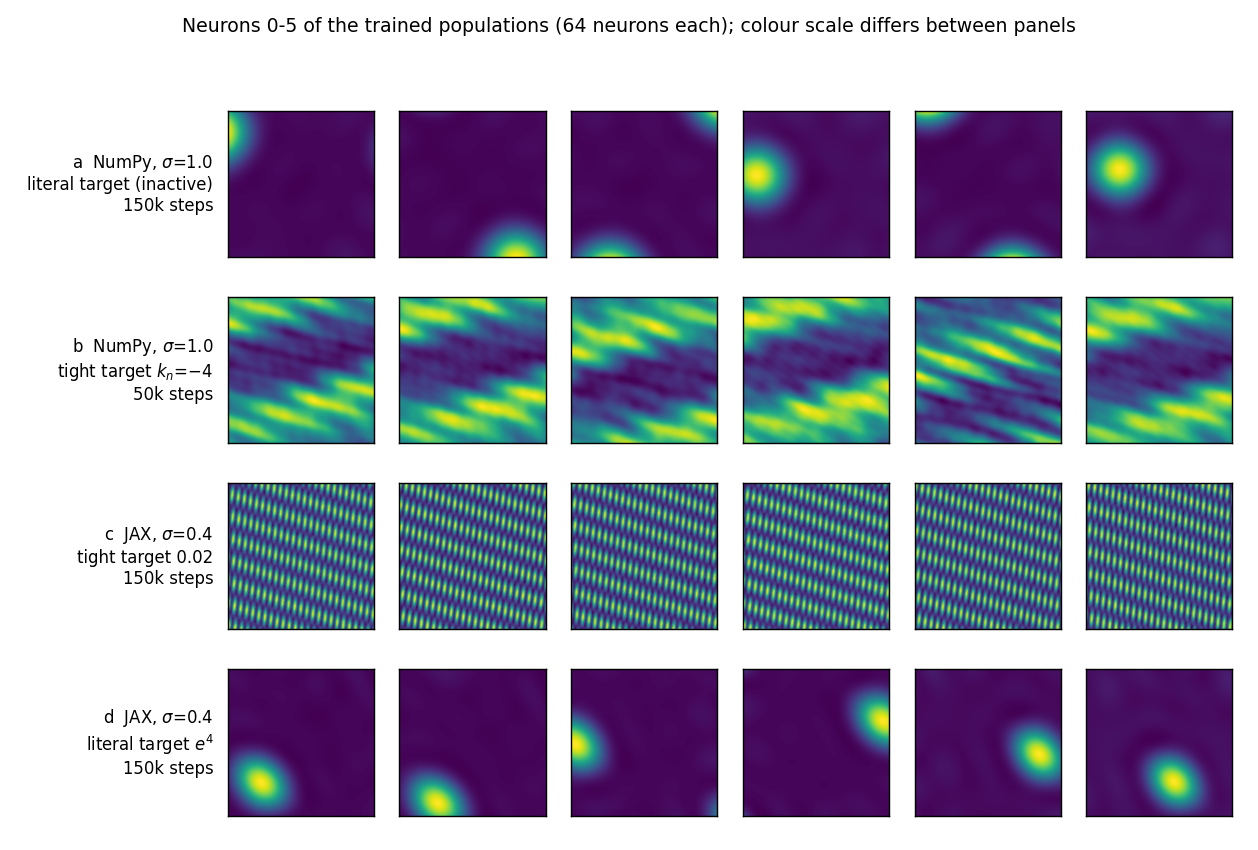
\includegraphics[width=0.58\linewidth]{figures/norm_target_montage.png}
\caption{Rate maps of neurons 0--5 under a literal and a tight norm target, in both implementations (window $[-1.5,1.5]^2$; colour scale differs between panels). Rows~a and~b are the NumPy runs at $\sigma=1.0$; the module in row~a is a hexagonal lattice of spacing \xSpacingLoose{} (from the autocorrelogram of the whole plane), larger than the window, and the module in row~b has spacing \xSpacingTight{} and is not hexagonal. Rows~c and~d are JAX seed-0 runs at $\sigma=0.4$.}
\label{fig:montage}
\end{figure}
\begin{figure}[H]
\centering
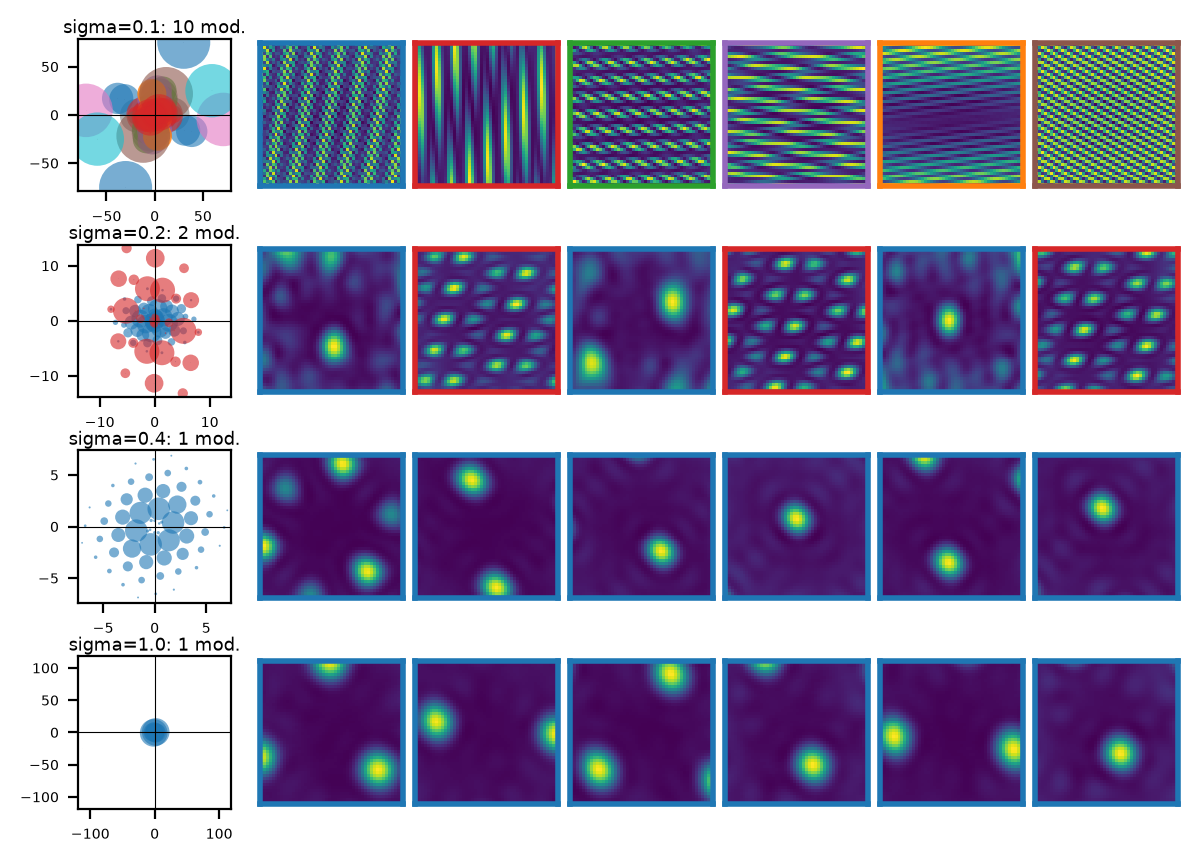
\includegraphics[width=0.52\linewidth]{figures/numpy_sigma_sweep.png}
\caption{NumPy implementation, $l=0.5$, 50k steps, seed 0: learned frequency power (left; one colour per module) and example rate maps (frame colour = module) at four values of $\sigma$. The module count falls from 10 at $\sigma=0.1$ to 1 at $\sigma=1.0$.}
\label{fig:sigma}
\end{figure}
\begin{figure}[H]
\centering
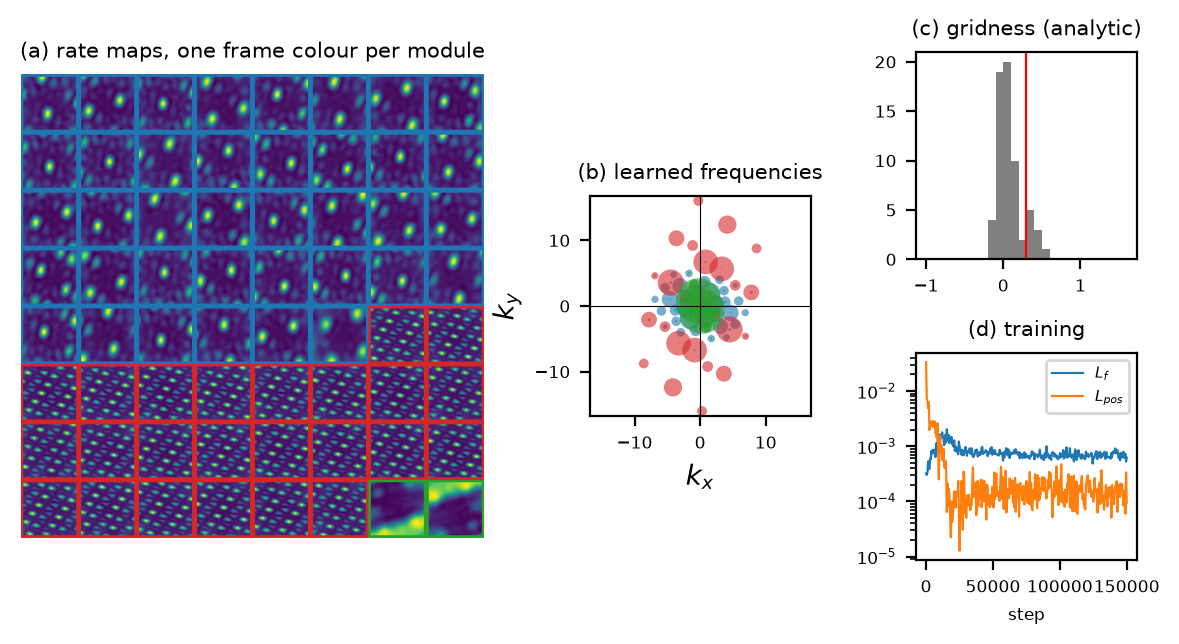
\includegraphics[width=0.66\linewidth]{figures/numpy_main_sigma02.png}
\caption{NumPy implementation at the settings of Figure~2B of the paper ($\sigma=0.2$, $l=0.5$, $N=64$, 150k steps, seed 0): (a) rate maps, one frame colour per module, (b) learned frequencies, (c) histogram of gridness (red line: 0.3), (d) training losses. The three modules are not hexagonal.}
\label{fig:main}
\end{figure}
\begin{figure}[H]
\centering
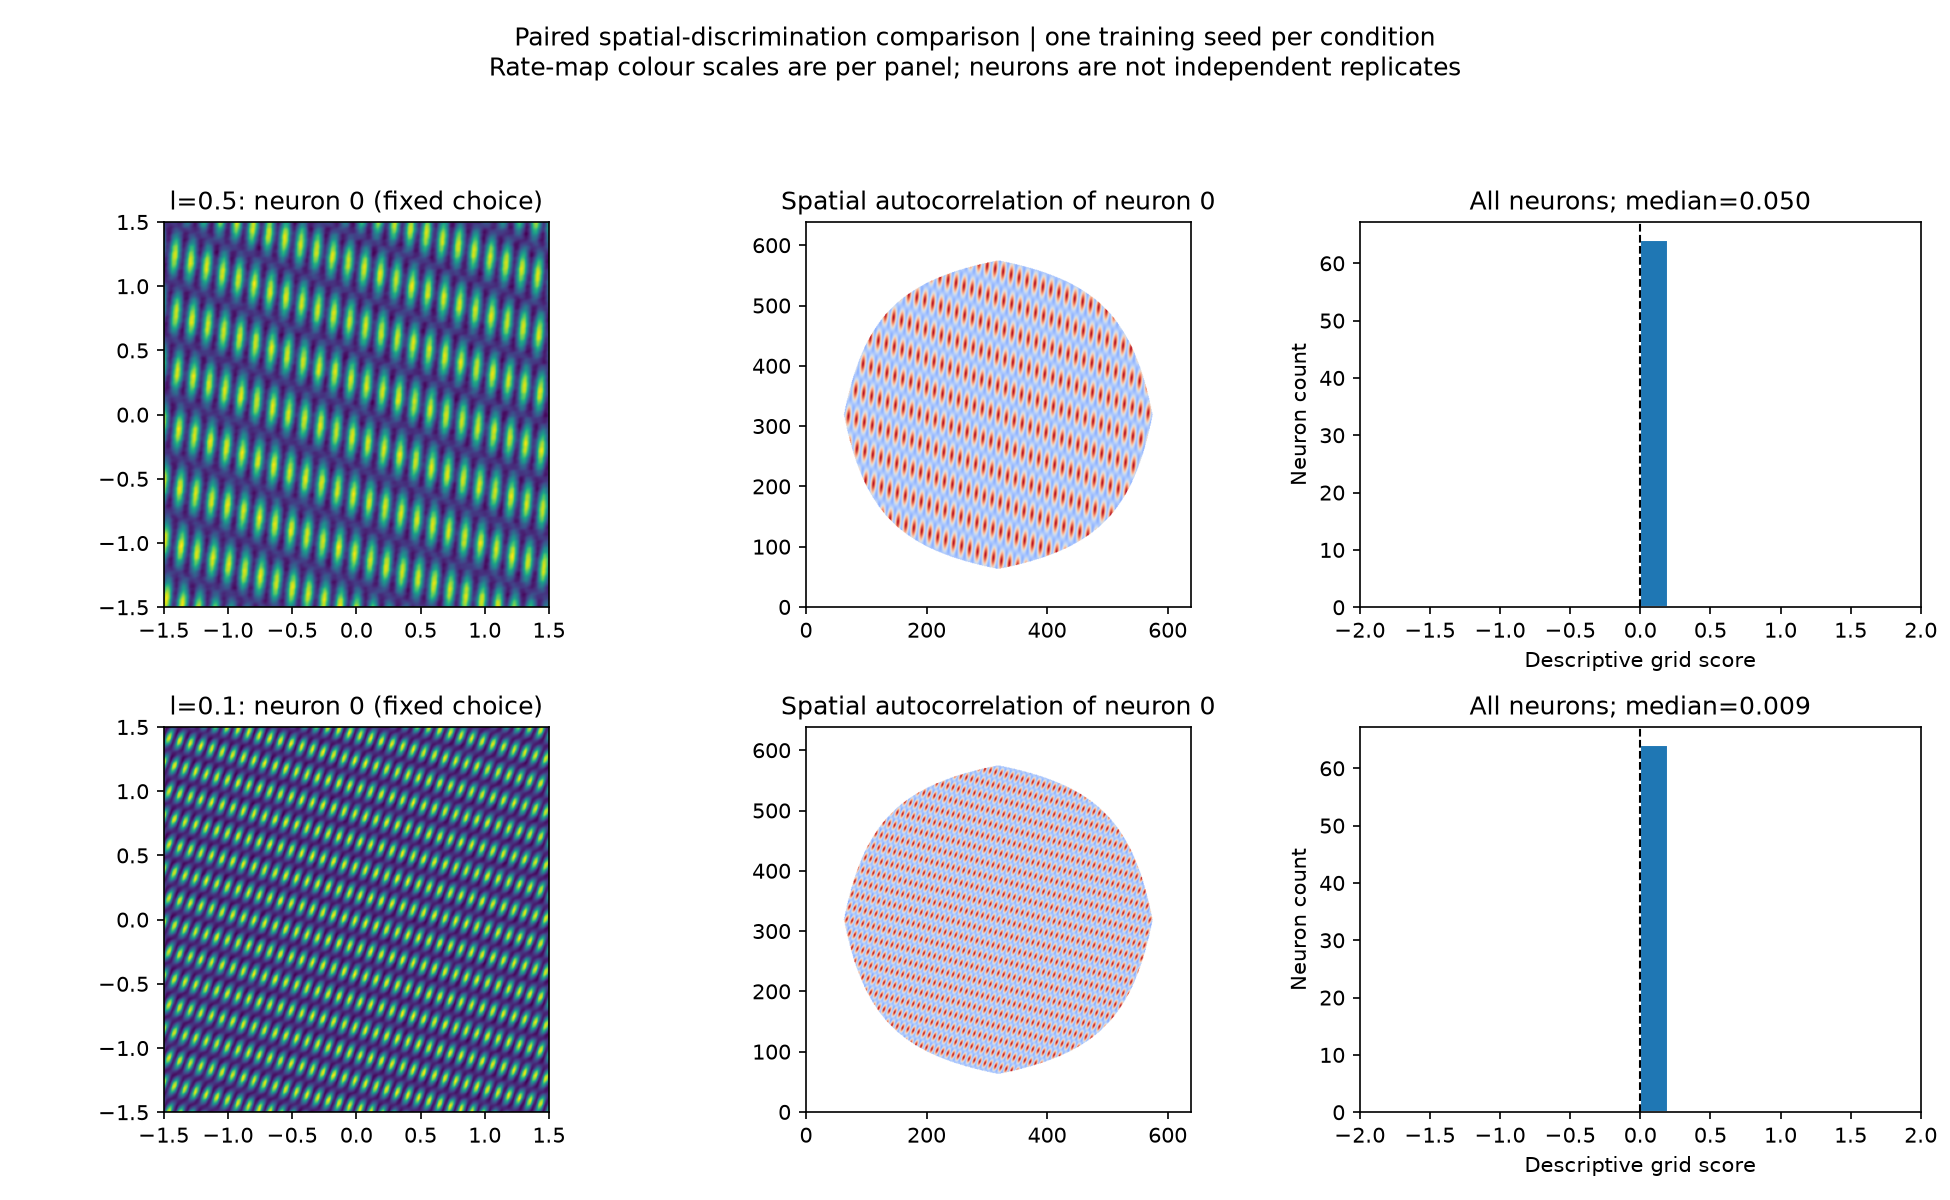
\includegraphics[width=0.7\linewidth]{figures/jax_comparison.png}
\caption{JAX implementation, the two seed-0 reference runs at $\sigma=0.4$ (150k steps): neuron 0, its spatial autocorrelation, and the distribution of descriptive grid scores over all 64 neurons, for $l=0.5$ (top) and $l=0.1$ (bottom). Rate-map colour scales differ between panels; neurons are not independent replicates.}
\label{fig:jaxcomp}
\end{figure}
\begin{figure}[H]
\centering
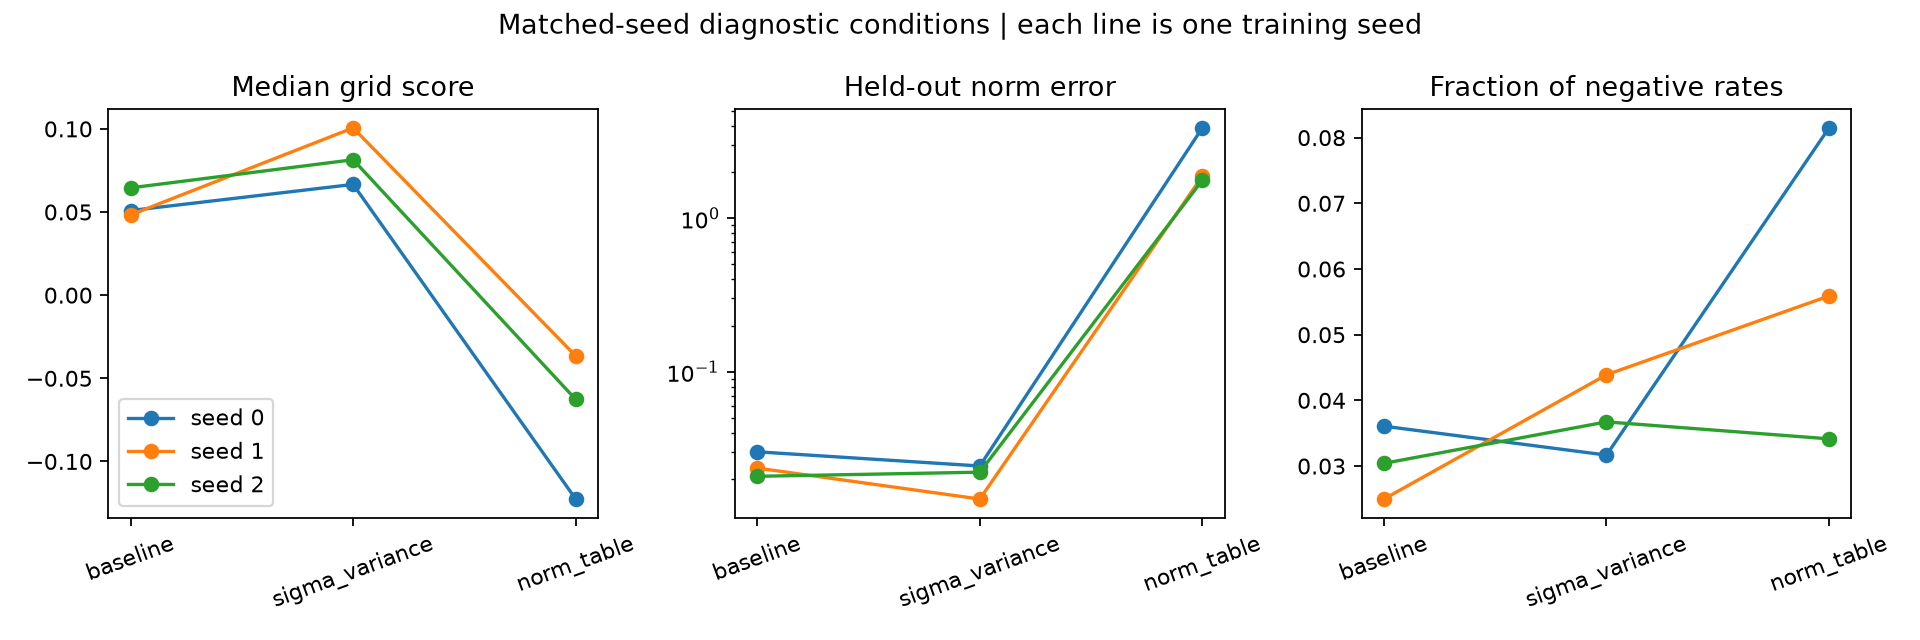
\includegraphics[width=0.88\linewidth]{figures/jax_diagnostics.png}
\caption{JAX implementation: all nine diagnostic checkpoints (150k steps each; lines connect matched seeds, initial states identical within a seed). Only the named setting changes: baseline uses $\sigma=0.4$ and norm target 0.02; sigma\_variance uses $\sigma=\sqrt{0.4}$; norm\_table uses the literal norm target $e^{4}$. All evaluations use one common grid and held-out samples; negative rates are those below $-10^{-6}$; the norm axis is logarithmic.}
\label{fig:diag}
\end{figure}
\begin{figure}[H]
\centering
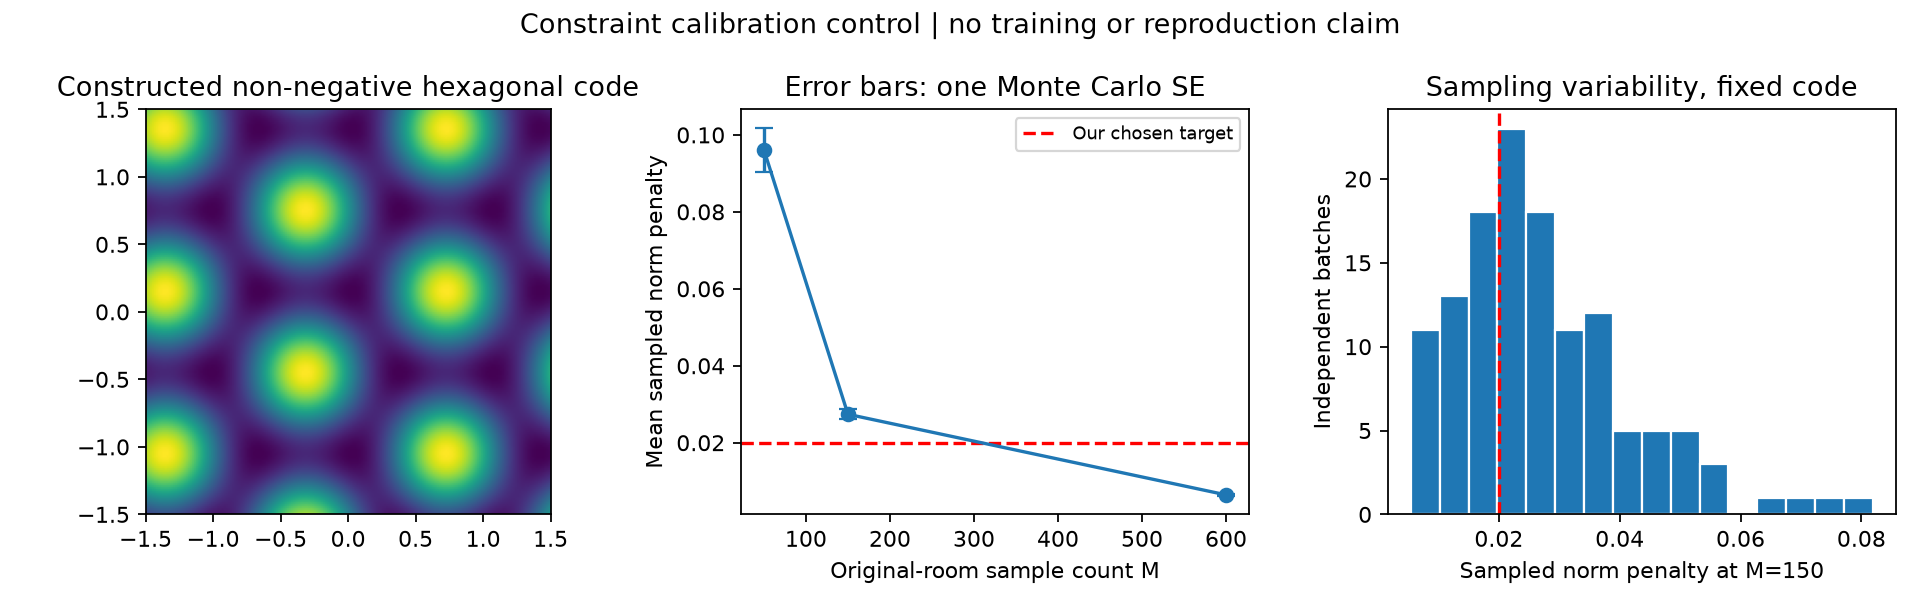
\includegraphics[width=0.88\linewidth]{figures/jax_constraint_control.png}
\caption{JAX implementation, constructed-code control (no training). Left: one neuron of a deliberately constructed non-negative hexagonal population. Centre: the sampled norm penalty falls as more positions are used to estimate room energy (error bars: one standard error over 128 sampling batches). Right: the distribution at 150 points; the 0.02 target is exceeded in most batches although the geometry is valid.}
\label{fig:control}
\end{figure}

\clearpage
\section*{NeurIPS checklist: reproduction submission}
\noindent Answers apply to our reproduction code (both implementations), not to Dorrell et al.'s paper. The questions are abbreviated and paraphrased from the \href{https://neurips.cc/public/guides/PaperChecklist}{NeurIPS checklist}.
\begin{enumerate}[leftmargin=1.6em,itemsep=2pt]\raggedright
\item \textbf{Are the claims supported and appropriately scoped? Yes.} The review separates the paper's claims, our reproduction and proposed follow-up work. We claim no successful reproduction of Figure~2B or Figure~8; Table~\ref{tab:verdict} shows which claims held.
\item \textbf{Are limitations explained? Yes.} The Reproducibility section reports the seeds, step budgets, our own thresholds for ``module'' and ``hexagonal'', the tolerance choices, and what was not attempted.
\item \textbf{Are new theoretical claims proved? N/A.} We introduce no theorem; the reviewed theory is attributed to Dorrell et al.
\item \textbf{Can the numerical findings be checked? Yes.} Both implementations ship configurations, seeds, saved runs (NumPy: parameters and metrics of all \nJobs{} runs; JAX: checkpoints, metadata and evaluation summaries), unit tests, and a quick check, \texttt{smoke\_test.py}. Every number in the review is a macro generated from these files.
\item \textbf{Are code, inputs, and instructions available? Yes.} The submitted archive contains all code, results, \texttt{README.txt} and \texttt{requirements.txt}. Positions are synthetic samples generated from recorded seeds; no external dataset is needed.
\item \textbf{Are experimental choices documented? Yes.} \texttt{numpy\_impl/README.txt} and \texttt{jax\_impl/references/implementation\_notes.md} list the sampling scheme, budgets, optimiser, targets, and every choice the paper leaves open. A configuration accompanies each run.
\item \textbf{Is uncertainty quantified statistically? No (partly).} Most settings have one to three seeds. The 50k-step baseline has \baseSeeds{} seeds (mean $\pm$ SD) and the scaling slope has a bootstrap interval. Neurons are not treated as independent runs, and grid scores are descriptive, without shuffled significance tests.
\item \textbf{Are computing requirements fully reported? Partly.} NumPy: about \xCpuHours{} CPU-hours for all \nJobs{} runs on a PC (a 150k-step run takes about \trainMinLong{} minutes). JAX: about \jRefMinutes{} minutes per reference run (the two ran concurrently) and \jDiagMinutes{} minutes of training time summed over the nine diagnostic runs. CPU only. Peak memory and total preliminary compute were not measured.
\item \textbf{Does the research conform to the NeurIPS Code of Ethics? Yes.} We ran no human or animal experiments and used only simulated data.
\item \textbf{Are application-specific societal risks discussed? N/A.} This is a small synthetic modelling exercise with no deployed application or personal data. The relevant risk is scientific over-interpretation, addressed by explicit limits on our claims.
\item \textbf{Are special release safeguards required? N/A.} The released artefacts are a small spatial-representation model and synthetic numerical results.
\item \textbf{Are asset licences respected? Yes for third-party assets; our own code has no licence file.} NumPy, SciPy, Matplotlib and JAX are used through \texttt{pip} under their own licences, the course style file is used as supplied, and no code from the authors' repository is copied. A licence for our code would have to be added before any upstream contribution.
\item \textbf{Are new artefacts documented? Partly.} Methods, configurations, tests and limitations are documented in both implementations; redistribution licensing is unresolved.
\item \textbf{Are human-participant instructions and compensation described? N/A.} No participants or crowdworkers were recruited.
\item \textbf{Was ethics approval obtained where needed? N/A.} No human-subject research was performed and no animal data were collected.
\item \textbf{Is substantive LLM use disclosed? Yes.} ``Author contributions and AI use'' states which assistant wrote which code and text; the Wits Science Faculty AI declaration accompanies the submission.
\end{enumerate}

\end{document}
